%% LyX 2.0.4 created this file.  For more info, see http://www.lyx.org/.
%% Do not edit unless you really know what you are doing.
\documentclass[11pt,onecolumn]{amsart}
\usepackage[T1]{fontenc}
\usepackage[latin9]{inputenc}
\usepackage{amsthm}
\usepackage{listings}
\usepackage{xcolor}
\usepackage{textcomp}
\usepackage{graphicx}

\makeatletter
%%%%%%%%%%%%%%%%%%%%%%%%%%%%%% Textclass specific LaTeX commands.
\numberwithin{equation}{section}
\numberwithin{figure}{section}

\newcommand{\be}{\begin{equation}}
\newcommand{\ee}{\end{equation}}
\newcommand{\mb}[1]{\mathbf{#1}}
\newcommand{\ut}[1]{\,\mathrm{#1}}

%%%%%%%%%%%%%%%%%%%%%%%%%%%%%% User specified LaTeX commands.

\usepackage{amsthm}\usepackage{amstext}\usepackage{setspace}
\usepackage[margin=0.5in, top=1in]{geometry}
\lstset{
        tabsize=4,
        language=MATLAB,
        basicstyle=\scriptsize,
        %upquote=true,
        aboveskip={1.5\baselineskip},
        columns=fixed,
        showstringspaces=false,
        extendedchars=true,
        breaklines=true,
        prebreak = \raisebox{0ex}[0ex][0ex]{\ensuremath{\hookleftarrow}},
        frame=single,
        showtabs=false,
        showspaces=false,
        showstringspaces=false,
        identifierstyle=\ttfamily,
        keywordstyle=\color[rgb]{0,0,1},
        commentstyle=\color[rgb]{0.133,0.545,0.133},
        stringstyle=\color[rgb]{0.627,0.126,0.941},
}
%%%%%%%%%%%%%%%%%%%%%%%%%%%%

\makeatother


\begin{document}

\title{Problem  B - Optimal Diameter of Table Tennis Balls for Spectator Enjoyment}


\author{Team 463}
\begin{abstract}
\fontsize{11}{12}\selectfont
In this paper we analyze the effect of increasing the diameter of a table tennis ball on its trajectory while rallying, and how it relates to the enjoyment of spectators. We define spectator enjoyment based on the speed of the shot, as this relates to how easily the ball may be seen, and the spin of the shots, which contributes to the variety of the shots and thus variety of gameplay which is essential to the enjoyment of spectators. As the ball diameter increases, the speed of the shots decrease, as does the total spin. We find that a ball of diameter $44\ut{mm}$, maintains a balance of reduced speed of ease of observation by spectators, and sufficient spin to maintain shot complexity and variety.
 
\end{abstract}
\maketitle
\newpage

\markright{TEAM 463}


\twocolumn {
\section{Introduction}

Table tennis, since its inception into the 1988 Olympics, has been well known as a fast paced sport. In the past, table tennis has been played with a hard smooth paddle, making the use of spin in shots extremely difficult. Since the 1970s, the use of sponged rubber on table tennis paddles gained popularity. With these new paddles, the use of spin in conjunction with speed in table tennis became extremely prevalent, making the sport ever more exciting to watch \cite{HISTORY}.  \\

Recently however, more elastic paddles have made the game excessively fast and difficult to watch on television \cite{HISTORY}. Hence it is necessary to consider methods to slow down the game for general audiences. In this paper, we determine the effect of increasing radius as a method to slow down the game. \\

To define what a 'fun' game to watch would be, Team 463 visited a local table tennis tournament to gather the opinion of resident table tennis players. All players agreed that for a general audience, a slower game would be more fun to watch. However, many of them felt that a larger ball was more difficult to spin and thus resulted in a poorer game to watch. Hence, to make the game as fun to watch as possible, we analyze the effect of radius on both the speed and spin of the ball, reaching a compromise between the two.


\section{Theory and Assumptions}
        In order to simplify the question, the speed of the game was quantified by the duration of one rally (i.e. the length of time a ball takes to travel from one edge of the table to the other given some initial velocity, $\mb{v_0}$, and spin $\boldsymbol{\omega_0}$). The rules of table tennis require that the ball travels over the net and bounce only once on the other side of the table. It is then natural to break the problem into two distinct parts, the in flight trajectory of the ball, and the rebound of the ball off the table. Following this, we may easily evaluate the time for a single shot by piecing the two solutions together. We present theoretical considerations for both these problems below. \\

\begin{figure}
\caption{Free Body Diagram of Table Tennis Ball in flight.  Here $\mb{F_G}$ represents the force of gravity, $\mb{F_M}$ the magnus force, $\mb{F_D}$ the drag, $\boldsymbol{\omega}$ is the angular velocity and $\mb{v}$ the velocity.}
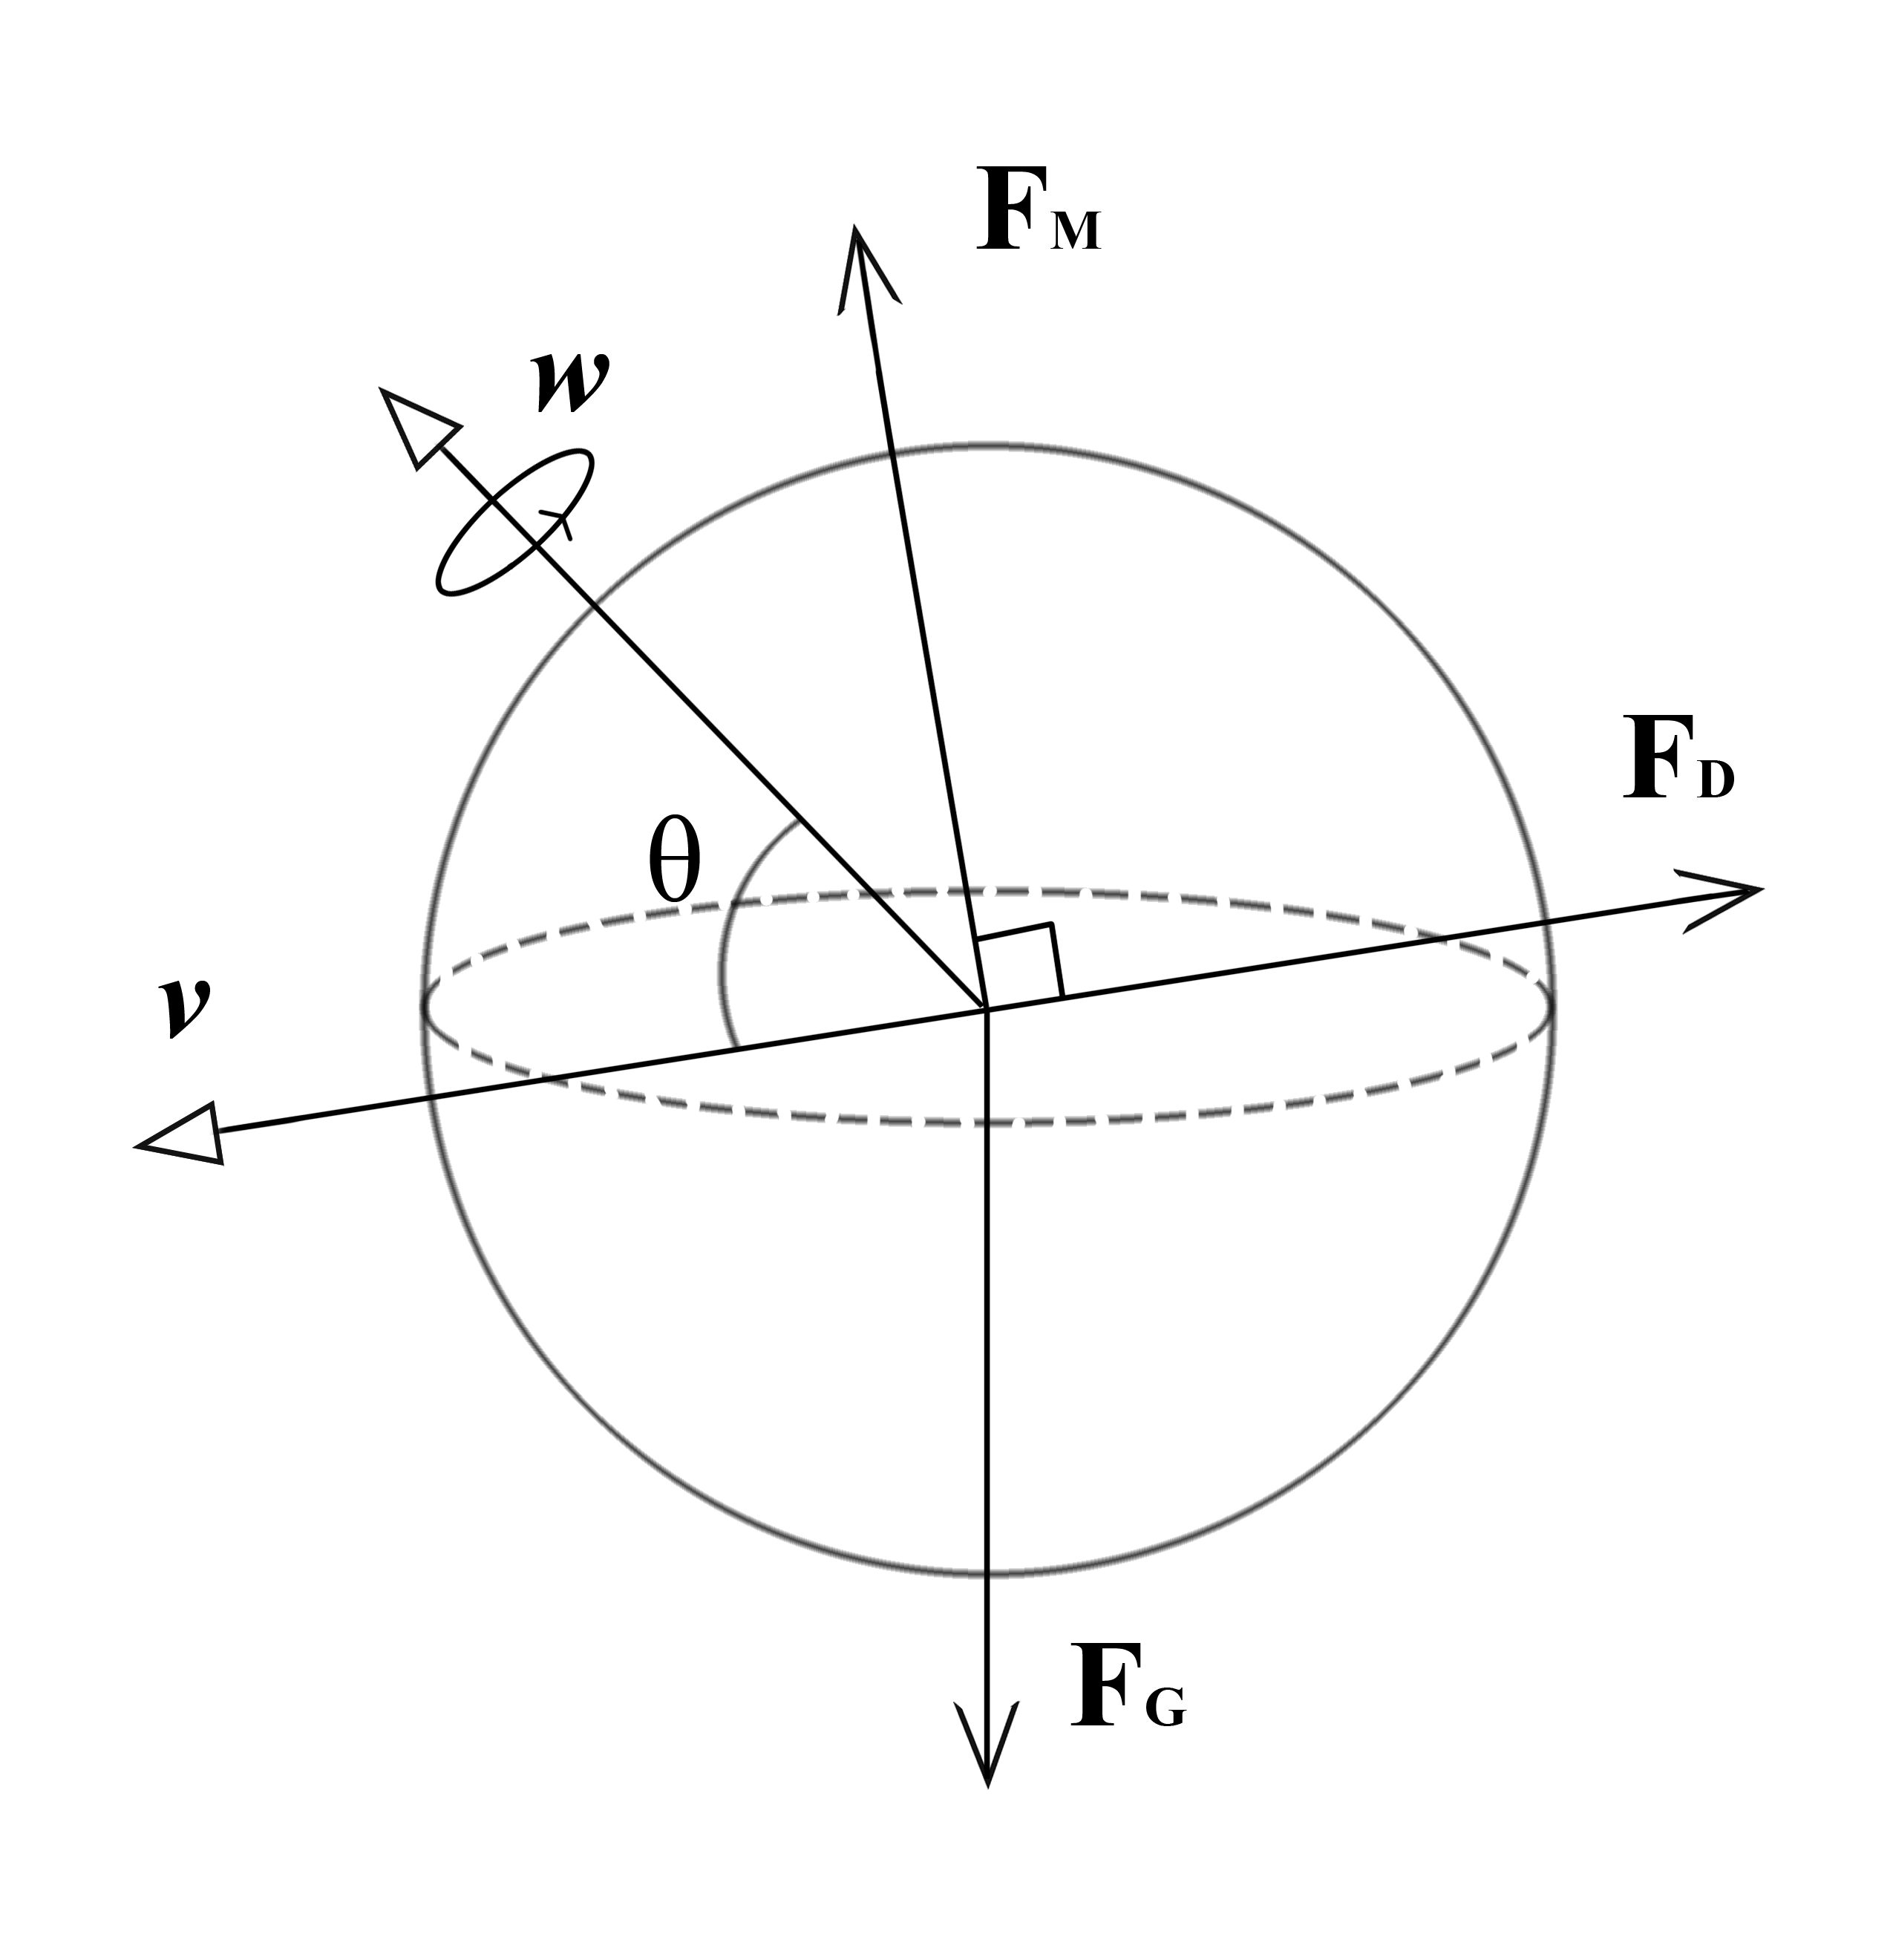
\includegraphics[width=0.5\textwidth]{figures/freebodypingpongball.png}
\label{pingpongball}
\end{figure}

\subsection{In Flight Trajectory}
To derive the in flight trajectory of the ping pong ball, we subject
it to three forces: gravity, drag by air resistance and Magnus force. 
The free body diagram of the ping pong ball is shown in \ref{pingpongball},
and we can use it to derive the differential equation governing the
trajectory. We can immediately consider the following equations,

\be
\mathbf{F}=\mathbf{F}_{G}+\mathbf{F}_{M}+\mathbf{F}_{D}
\ee
\be
\mathbf{F}_{G}=-m\cdot g\mathbf{\hat{k}}
\ee
\be
\mathbf{F}_{D}=-\frac{1}{2}\rho C_{D}(\pi R)^{2}||\mathbf{v}||\mathbf{v},
\ee

where \textbf{$\mathbf{F}_{G}$} accounts for gravity, and \textbf{$\mathbf{F}_{D}$} accounts for drag. We denote $m$ as the mass of the ball, $g$ as the acceleration due to gravity, $\rho$ as the air density, $C_{D}$ as the drag coefficient, and $R$ as the radius of the ball. To derive the Magnus force takes a little more effort. Using the Kutta-Joukowski Lift Theorem \cite{NASA1} for a cylinder, we find that

\be
\mathbf{F}_{M}=\rho(2\pi R)^{2}(\mathbf{\boldsymbol{\omega}}\times\mathbf{v}).
\ee
\\

Integrating along the axis of rotation, we find
\begin{align}
\mathbf{F}_{M} &= \int_{-R}^{R}\rho\left(2\pi \sqrt{R^{2}-x^{2}}\right)^{2}(\mathbf{\boldsymbol{\omega}}\times\mathbf{v})\mathop{\textnormal{dx}} \\
                      &= \frac{16}{3}\pi^{2}\rho R^{3}(\mathbf{\boldsymbol{\omega}}\times\mathbf{v}), \notag
\end{align}

which describes the Magnus force acting on a sphere. We then obtain the net force,

\begin{align}
\mathbf{F} = &-m g\mathbf{\hat{k}+}\frac{16}{3}\pi^{2}\rho R^{3}(\mathbf{\boldsymbol{\omega}}\times\mathbf{v}) \\
                 &-\frac{1}{2}\rho C_{D}(\pi R)^{2}||\mathbf{v}||\mathbf{v}. \notag
\end{align}



by taking the sum of the individual forces. We further assume that
the angular velocity is non-constant, and thus decreases over time
due to drag torque. We may use an analogous formula for the drag torque
found in \cite{RUSSIANS} where 
\be
\boldsymbol{\tau}_{D}=I\frac{d{\boldsymbol{\omega}}}{dt}=-\frac{1}{2}C_{\omega}\rho R^{5}||\boldsymbol{\omega}||\boldsymbol{\omega}.
\ee
When numerically solving these differential equations, we can also
adjust the rotational velocity in parallel to the main calculation, to account
for the decay in rotational velocity, and how it affects the Magnus force. \\


\begin{figure}
\caption{
Impluse during and velocities before and after the collision with table.  $\boldsymbol{\omega}$ and $\boldsymbol{\omega '}$ represent the angular velocity before and after respectively.  $\mb{v}$ and $\mb{v '}$ are likewise the velocities of the ball, and $\mb{u}$,  $\mb{u '}$ the contact velocities of the ball with the table.  
$\mb{J_fr}$ refers to the impulse due to friction with the table, and $\mb{J_z}$ is the z-component of impluse.
}

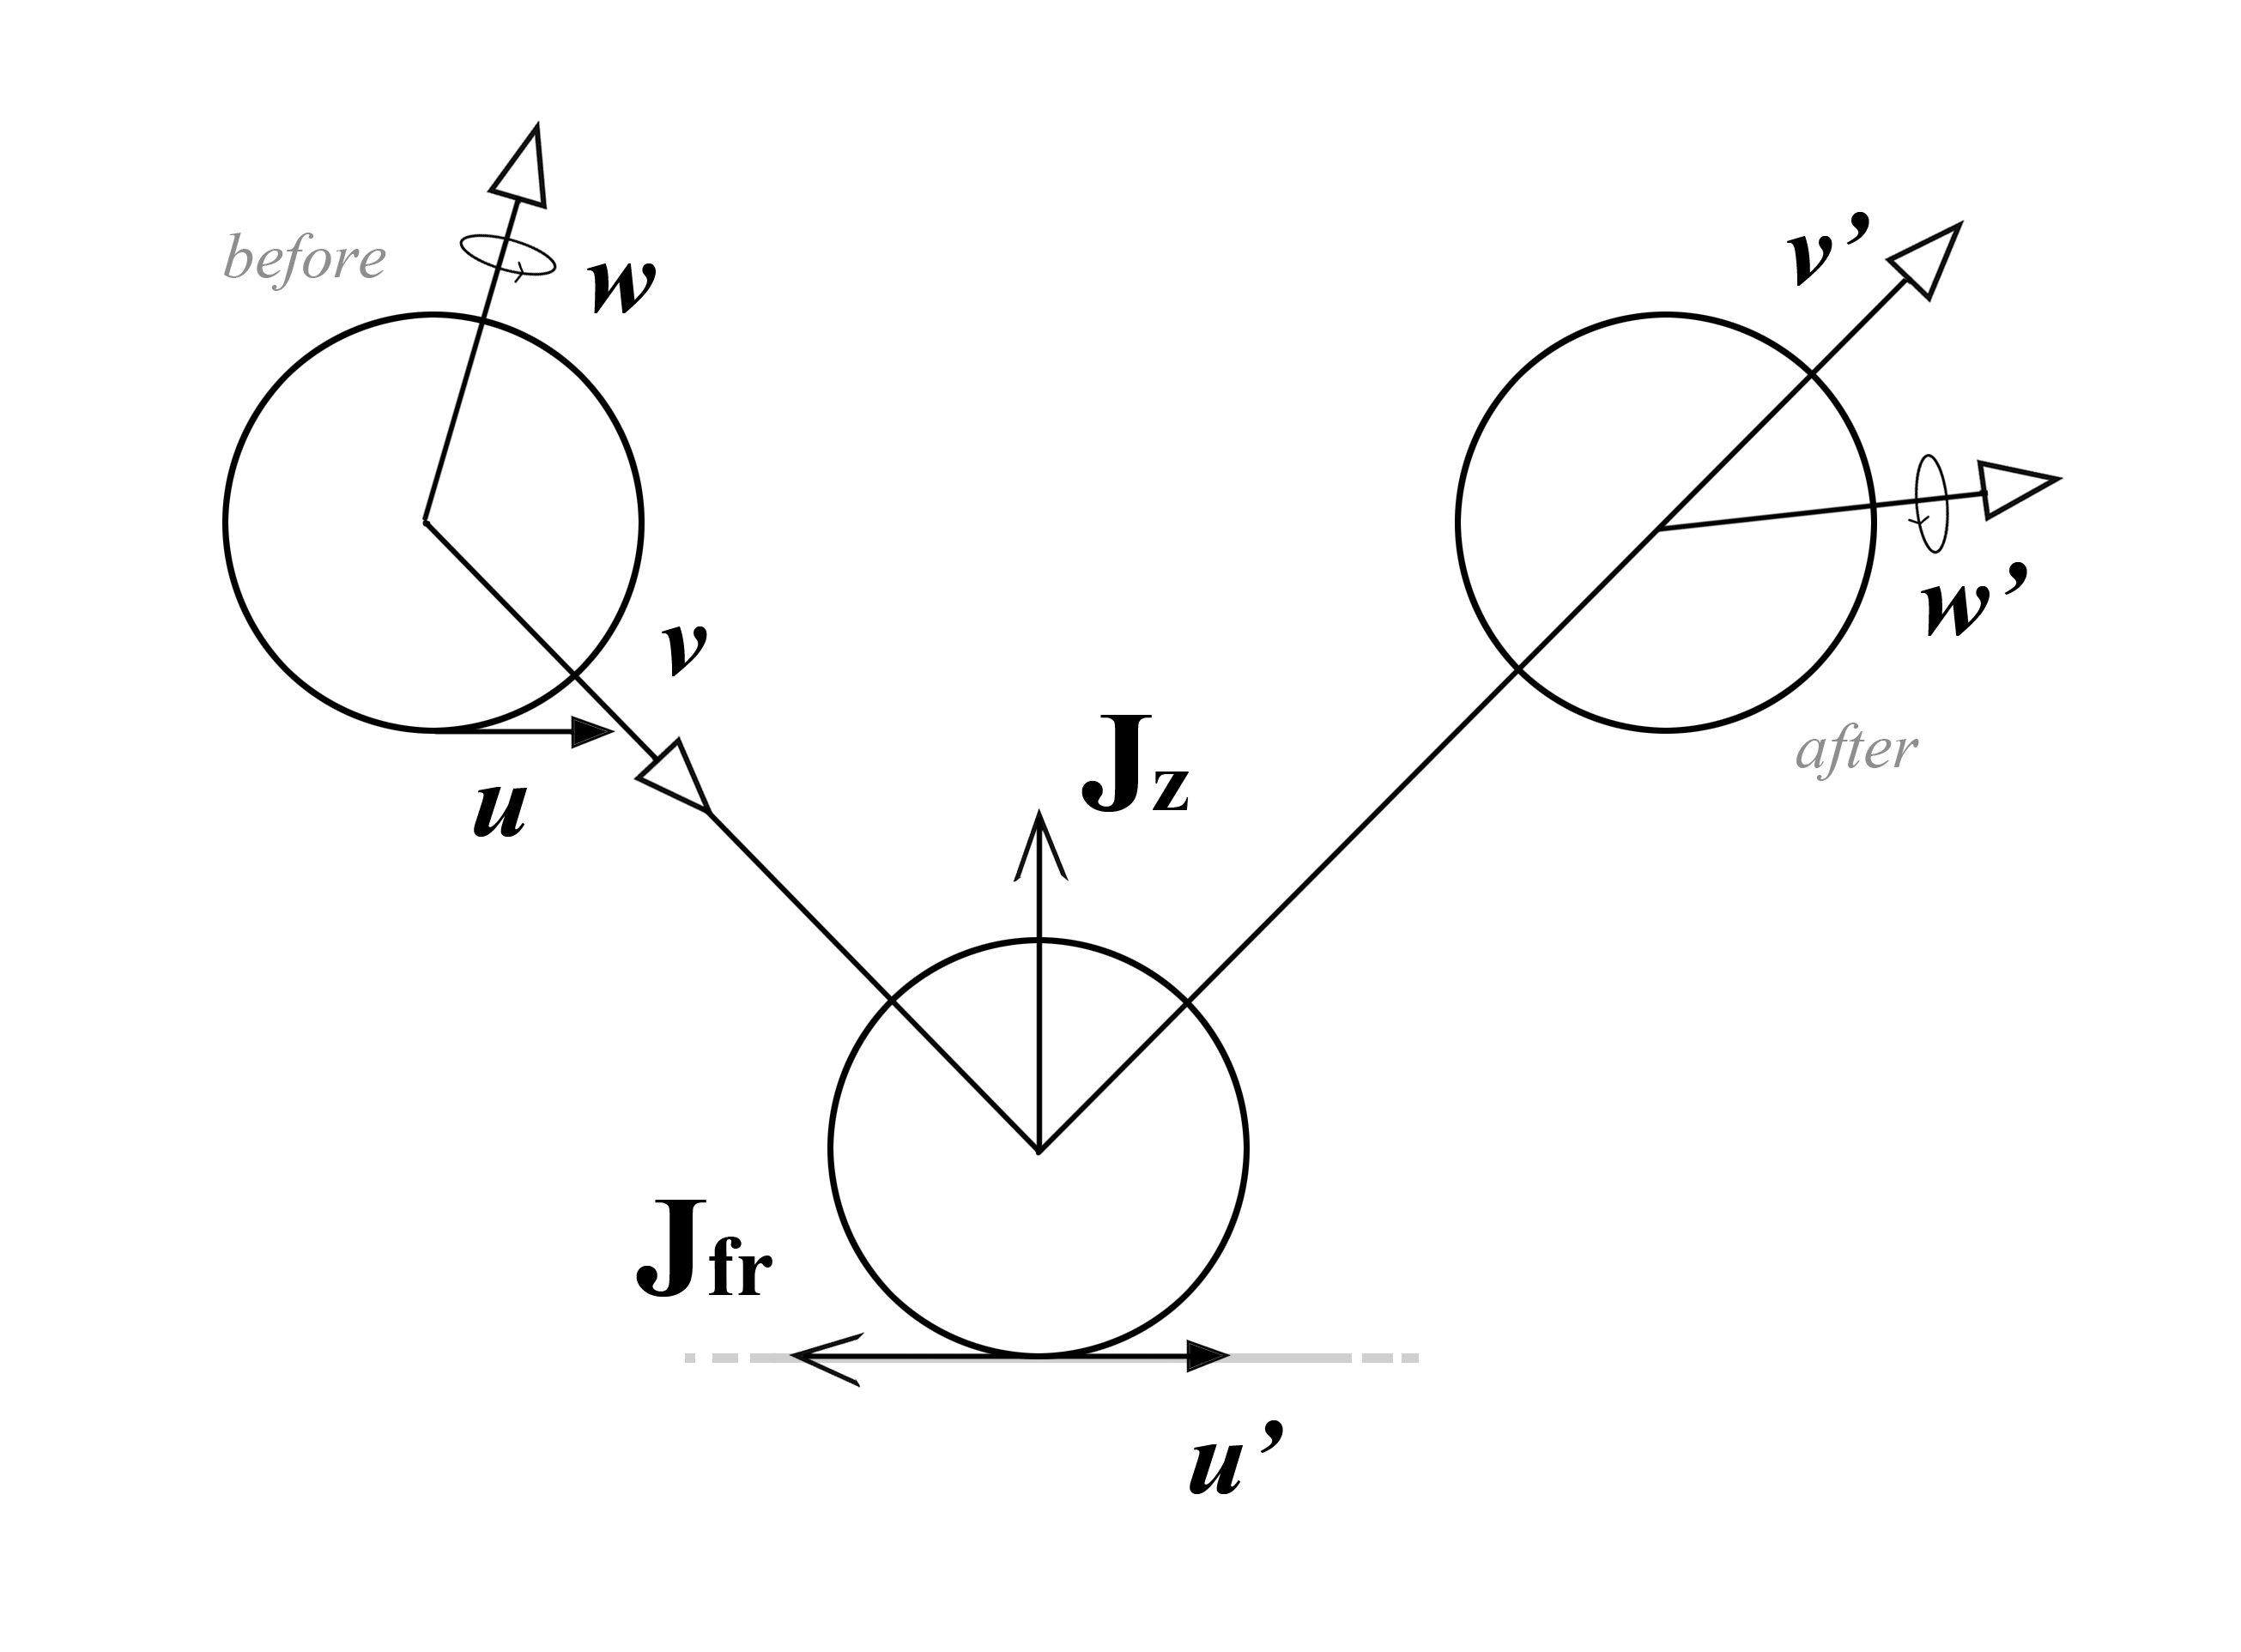
\includegraphics[width=0.5\textwidth]{figures/tablecollisiondiagram.png}
\label{tablehit}
\end{figure}

\subsection{Rebound of Ball on Table}
Due to friction as well as the deformation of the ball during play, we cannot expect a simple elastic collision when the ball hits the table. Instead we follow the model of, which has been verified experimentally to good accuracy \cite{MAIN}. For clarity, we give a quick derivation of the model below. \\

Let $\mathbf{v}$, $\mathbf{v'}$, $\boldsymbol{\omega}$ and $\boldsymbol{\omega'}$ be the velocity and angular velocity of the ball respectively, before and after collision. Let $u$ and $u'$ be the velocity of the contact point of the ball with the table \ref{tablehit}. It follows that:\footnote{All subscripted vectors in this paper refer to the subscripted components only.} 
\be
        \mathbf{u} = \mathbf{v_{xy}} + (\boldsymbol{\omega} \times \mathbf{r})
\ee

Since a table tennis ball is relatively rigid, we treat the ball as a rigid object. This assumption has been shown to be accurate experimentally by  \cite{MAIN}. In an inelastic collision, the vertical component of the ball is given by: 
\be
\label{eq:restitute}
         v_z = -\epsilon v_z',
\ee
where $\epsilon$ is the coefficient of restitution of the ball. \\


Let $\mb{J}$ be the impulse of imparted on the ball by the table and $\mu$ be the coefficient of sliding friction between the ball and the table. Since the impulse in the $z$-direction is directly proportional to the normal force, the frictional force (or proportionally the impulse in the $xy$ direction) is governed by:
\be
        \mathbf{J_{xy}} = -\mu J_z\frac{\mathbf{u}}{||\mathbf{u}||}.
\ee
Here we assume that $J_z$ is always positive since the ball will always rebound into the positive $z$ direction. \\

Let $m$, $r$, and $I = \frac{2}{3}mr^2$ be the mass, radius, and moment of inertia of the ball respectively. From the Impulse-Momentum theorem,
\be
\label{eq:lin-momen}
        m\mathbf{v'}-m\mathbf{v} = \mathbf{J},
\ee
\be
\label{eq:ang-momen}
        I\boldsymbol{\omega'}-I\boldsymbol{\omega} = \mb{r} \times \mb{J}.
\ee
\\

Considering \ref{eq:lin-momen} and \ref{eq:ang-momen} component-wise, we obtain two new equations:
\be
\label{eq:final-z-imp}
        J_z = -m(1+\epsilon)v_z
\ee
\be
\label{eq:combined-u-prime}
        \mb{u'} = -\mu J_z\left(\frac{1}{m} + \frac{r^2}{I}\right)\frac{\mb{u}}{||\mb{u}||} + \mb{u},
\ee
where $\mb{u'}$ is the velocity of the contact point right after the bounce.
\\

Since the contact time of the ball with the table is small, we may make the assumption that the direction of the $xy$ component of $\mb{v'}$ does not change until the ball leaves the table. Thus we have the proportionality relation: 
\be
\label{eq:para-vel}
        \mb{u'} = c\mb{v'}
\ee
while the ball is on the table.
\\

From \ref{eq:restitute}, \ref{eq:combined-u-prime}, and \ref{eq:para-vel}, we may determine $c$:
\be
\label{eq:final-c}
        c = 1 - \frac{5}{2}\mu\left(1+\epsilon \right) \frac{|v_z|}{||\mb{u}||} = 1-\frac{5}{2}\alpha,
\ee
where \[\alpha = \mu \left(1+\epsilon \right)\frac{|v_z|}{||\mb{u}||}. \]
By our assumption above (reference the direction assumption), we must have $c \geq 0$. \\

Using equations \ref{eq:lin-momen}, \ref{eq:ang-momen}, and \ref{eq:final-c}, we may write the relationship between $\mb{v}$ and $\mb{v'}$ compactly as: 
\be
        \mb{v'}= \mb{A_v}\mb{v}+ \mb{B_v}\boldsymbol{\omega},
\ee
\be
        \boldsymbol{\omega'} =\mb{ A_\omega } \mb{v}+ \mb{B_\omega} \boldsymbol{\omega}.
\ee
\\

Physically, the $c > 0$ case is the case of sliding friction, where there is no physical bound on the magnitude of $c$. 
\be
\mb{A_v}= 
 \begin{pmatrix}
  1-\alpha & 0            & 0 \\
  0            & 1-\alpha & 0 \\
  0            & 0            & -\epsilon
 \end{pmatrix},
\mb{B_v}= 
 \begin{pmatrix}
  0 & \alpha r           & 0 \\
  -\alpha r           & 0 & 0 \\
  0            & 0            & 0
 \end{pmatrix},
\ee

\be
\mb{A_\omega} = 
 \begin{pmatrix}
 0 & -\frac{3\alpha}{2r}           & 0 \\
 \frac{3\alpha}{2r}           & 0 & 0 \\
  0            & 0            & 0
 \end{pmatrix},
\mb{B_\omega} = 
 \begin{pmatrix}
  1-\frac{3\alpha}{2}  & 0            & 0 \\
  0            & 1-\frac{3\alpha}{2} & 0 \\
  0            & 0            & 1
 \end{pmatrix},
\ee


Physically, the $c \leq 0$ case corresponds to rolling friction. By assumption, $\mb{u'}$ must be parallel to $\mb{u}$. Hence, the minimum physical $c$ corresponds to $\mb{u'} = \mb{0}$ (when the ball is purely rolling). Hence, $\alpha = \frac{2}{5}$. 

Since the rolling case is a limiting case of zero slide, we have:
\be
\mb{A_v}= 
 \begin{pmatrix}
 \frac{3}{5} & 0            & 0 \\
  0            & \frac{3}{5} & 0 \\
  0            & 0            & -\epsilon
 \end{pmatrix}
\mb{B_v}= 
 \begin{pmatrix}
  0 & \frac{2}{5} r           & 0 \\
  -\frac{2}{5} r           & 0 & 0 \\
  0            & 0            & 0
 \end{pmatrix}
\ee

\be
\mb{A_\omega} = 
 \begin{pmatrix}
 0 & -\frac{3}{5r}           & 0 \\
 \frac{3}{5r}           & 0 & 0 \\
  0            & 0            & 0
 \end{pmatrix},
\mb{B_\omega} = 
 \begin{pmatrix}
  \frac{2}{5}  & 0            & 0 \\
  0            & \frac{2}{5} & 0 \\
  0            & 0            & 1
 \end{pmatrix},
\ee

\subsection{Estimation of spin and shot time}
First, let us define a valid shot as a shot that goes over the net and bounces once on the other side.
From our results above, we may obtain the complete motion of a single valid table tennis shot. We may determine both the total time, $t$ over the entire motion, as well as the total path length, $\ell$. Furthermore, we reason that $\ell$ is a good indicator of spin, as a greater spin leads to a greater effect from the Magnus force, and hence a larger in flight distance. \\

By averaging $\ell$ and $t$ over all valid shots due to initial conditions for a particular radius, we can measure both spin and shot time efficiently. These computations are simple to do numerically and are described in the follow section.


\section{Numerical Implementation}
The motion of the ball was solved numerically using Matlab's ODE suite, by breaking the problem into motion before and after the bounce \ref{normal}. If the motion of the ball did not constitute a valid shot as defined previously, then the test was discarded. The simulation for a valid shot was stopped when
\begin{itemize}
        \item the ball either hit the table a second time or
        \item went out of the table. 
\end{itemize}

To determine $t$ and $\ell$ for a given radius, we may use a Monte Carlo method to simulate randomly over all possible shots using several initial speeds and spins. However, due to time constraints and the speed of the Monte Carlo simulation, we assumed that the ball was always hit from a fixed location across all simulations. This removes 3 dimensions of the simulation. For a given radius of the ball, the Monte Carlo assumed a constant energy and calculated the initial speed and angular speed accordingly. The estimate for energy was obtained from \ref{ITTF-STATS}, which gives the speed of one of the fastest table tennis shots ever recorded. We assume that this record shot had purely translational energy and use this energy as the maximum energy a table tennis ball can attain. Additionally, it was assumed that the typical shot would have approximately half of the total energy going into angular velocity and the other half going into translational velocity. Hence $\mb{v}$ and $\boldsymbol{\omega}$ follows:
\be
||\mb{v}|| = \sqrt{\frac{E_{max}}{m}}
\ee
\be
||\boldsymbol{\omega}|| = \sqrt{\frac{E_{max}}{I}}
\ee

By keeping $E_{max}$ constant, we may determine the typical speed and angular velocity for any single radius. We can then do a Monte Carlo simulation over all possible directions of the initial velocity and angular velocity. In polar coordinates, this means we take uniform samples over $\phi$ and $\theta$, where $\phi$ is the zenith angle and $\theta$ is the azimuthal angle on the $xy$-plane. Hence, the initial velocity and angular velocity is:
\be
\mb{v} = ||\mb{v}|| (\sin \phi_1 \cos \theta_1, \sin \phi_1 \sin \theta_1, \cos \phi_1),
\ee
\be
\boldsymbol{\omega} = ||\boldsymbol{\omega}|| (\sin \phi_2 \cos \theta_2, \sin \phi_2 \sin \theta_2, \cos \phi_2).
\ee
From this point we evaluate the effect of changing the radius by performing several simulations over various radii. \\

To obtain an accurate model, several parameters in the simulation were estimated:

The dimensions of the table were obtained from the International Table Tennis Federation \cite{ITTF}. We always assume that the ball is shot at $0.4\ut{m}$ above the surface of the table, as this height is the average height at which a table tennis ball is typically hit during play \cite{HEIGHT}. A diagram of the model setup is shown in \ref{table} \\


\begin{figure}
\caption{Table coordinate system used and dimensions.}
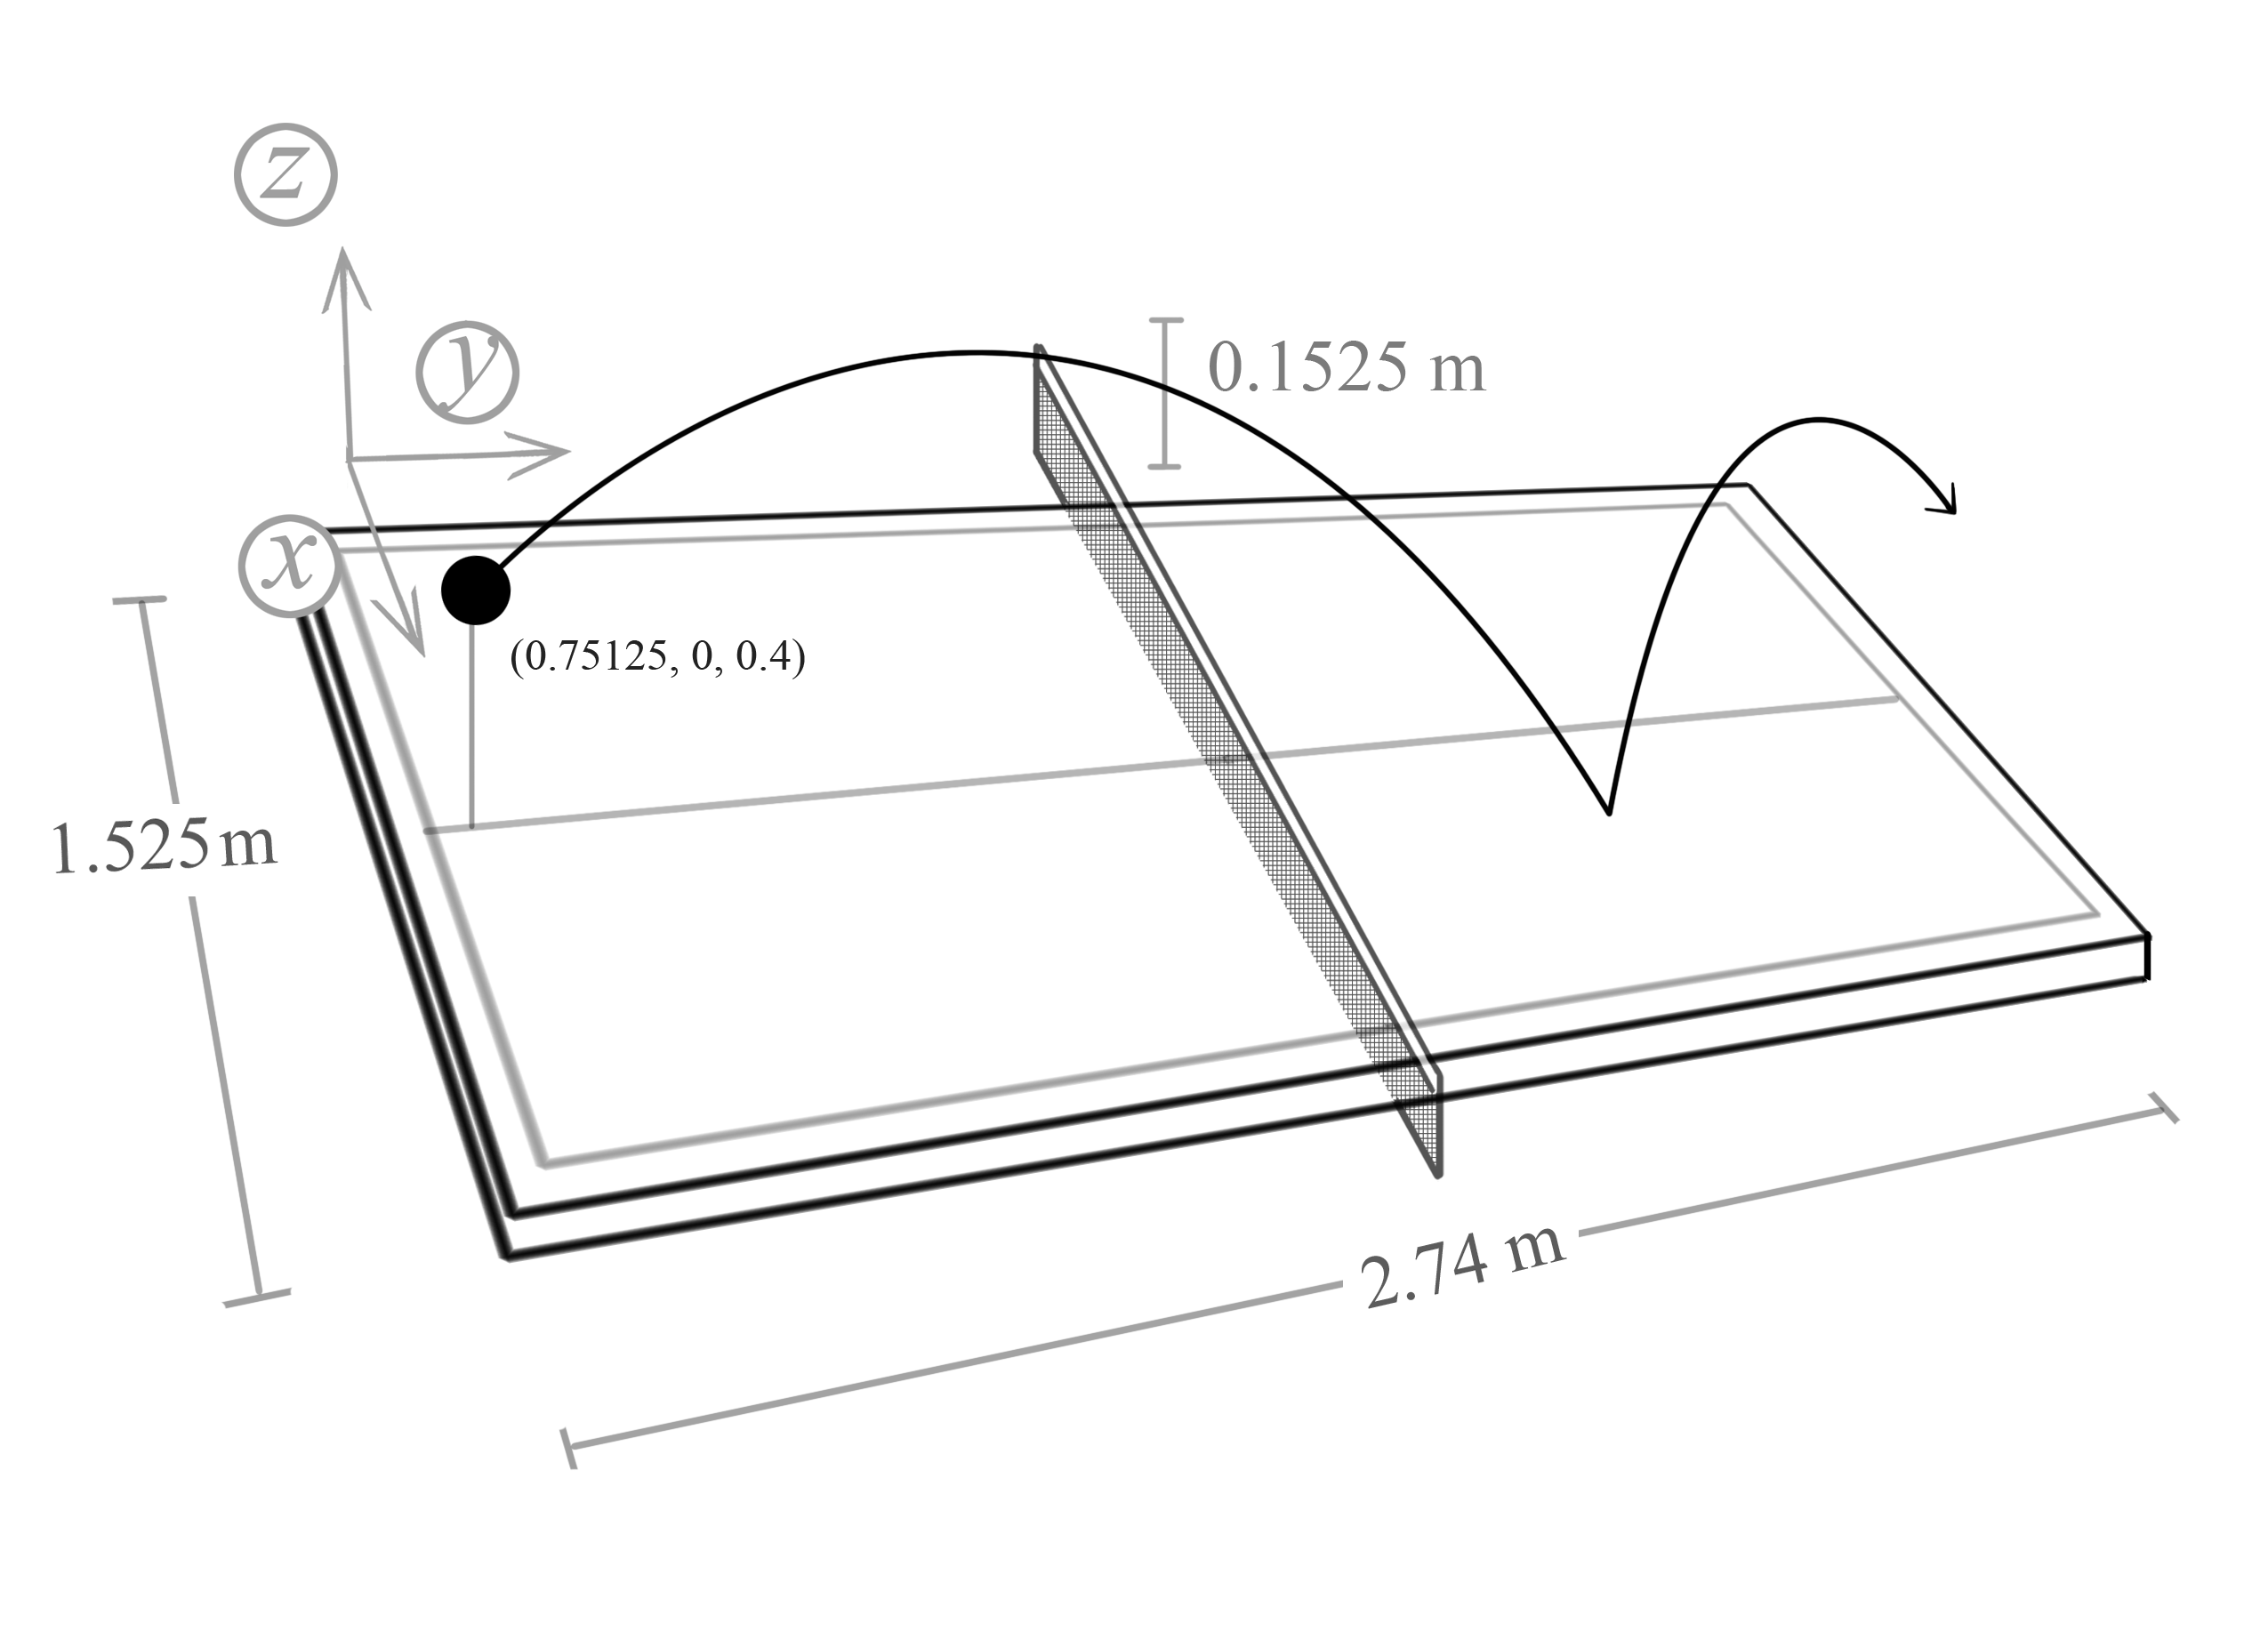
\includegraphics[width=0.5\textwidth]{figures/tablediagram.png}
\label{table}
\end{figure}


For the in flight portion of the shot, the important forces to consider were gravity, drag and the Magnus force which cases the lift when the ball spins. We estimate the mass of the ball by considering a fixed mass per area of the ball. From \cite{ITTF}, we use 2.7$\ut{g}$ for the 0.40$\ut{mm}$ diameter. Gravity can be estimated to be $9.8\,\mathrm{ms^{-2}}$. For the drag, we required an estimation of the drag coefficient for a hollow sphere, which we took to be 0.5. This value falls within the estimated range in literature \cite{NASA1}. Since the drag coefficient is dependent on the Reynolds number, taking it to be constant is a simplification. However, literature suggests that at higher Reynolds numbers, the drag constant stays roughly the same \cite{WIKI}. \\


\begin{figure}
\caption{Backspin shot moving left, with $\boldsymbol{\omega}$ = (100,0,0), $\boldsymbol{v} = (0,15,0)$, and no spin decay. This is clearly non-physical, but would make for a very exciting spectator sport.}
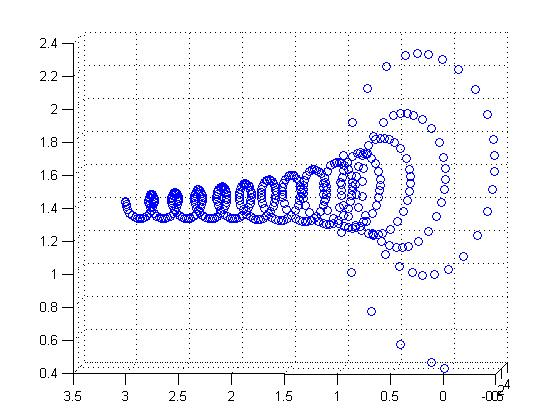
\includegraphics[width=0.5\textwidth]{sections/WeaknessesOfTheModel/WeaknessesOfOurModel.jpg}

\label{spiral}

\end{figure}

\begin{figure}
\caption{Simulation of average top spin shot. The red spheres represent the trajectory of the ball before the bounce.}
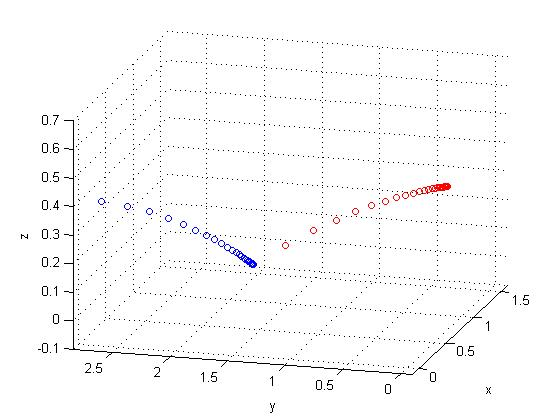
\includegraphics[width=0.5\textwidth]{figures/topspin.jpg}

\label{normal}

\end{figure}

Without considering a drag torque in the spin of the ball, the Magnus force dominates the in flight motion. Since the ball is light, and substantial spin can be delivered to the ball by a well trained player. Without considering decay, the model is highly unrealistic \ref{spiral}.  Using \cite{RUSSIANS}, we amended the angular velocity at every iteration of the DE solver, whose differential equation was analogous to that of translational drag. The value of $C_{\omega}$ was considered by \cite{FORCE}, which demonstrated a formula for $C_{\omega}$ with an error of $o(Re)$. Since the work of \cite{FORCE} was based on a small Reynolds number approximation, the assumption is less valid for a ball with substantial spin. Hence, the $o(Re)$ error term begins to dominate, which was the main factor in our equation when estimating $C_{\omega}$. The rotational drag coefficient was assumed to be a linear function of the rotational Reynolds number, for which \cite{WIKI} gave an approximate formula. The resulting simulation is much more realistic, though not as visually appealing, as seen in \ref{normal}.

\section{Results}

\begin{figure}
\caption{Average path length of shot for varying radii with input E = 0.39J.}
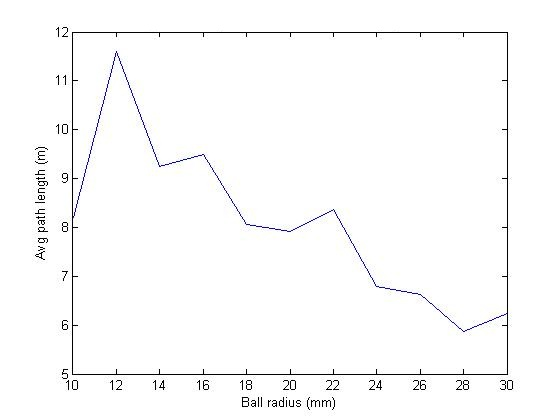
\includegraphics[width=0.5\textwidth]{figures/AvgPathLength.jpg}

\label{avgPathLength}

\end{figure}

\begin{figure}
\caption{Average velocity of shot for varying radii with input E = 0.39J.}
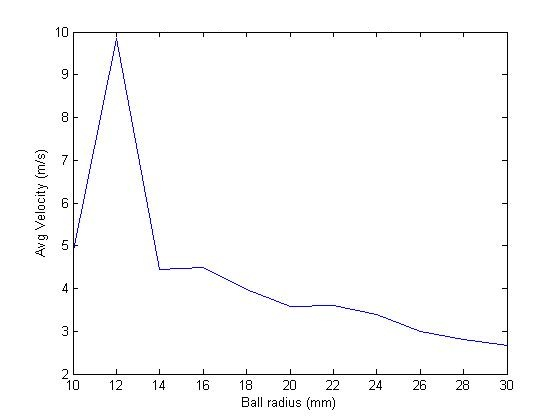
\includegraphics[width=0.5\textwidth]{figures/AvgVel.jpg}

\label{avgVel}

\end{figure}

\begin{figure}
\caption{Average time for shot to make it to the other end of the table, for varying radii with input E = 0.39J.}
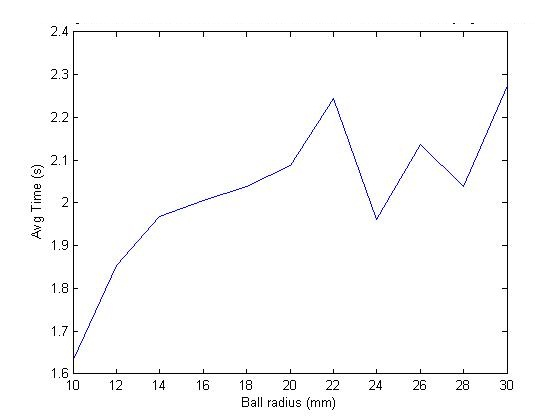
\includegraphics[width=0.5\textwidth]{figures/AvgTime.jpg}

\label{avgTime}

\end{figure}

Let the average time, and path length for a given radius be $t_{av}$ and $\ell+{av}$ respectively. Our model shows that as the radius of the ball increases, $t_{av}$, increases and $\ell_{av}$ decreases. Moreover, the average speed, calculated by averaging $\frac{\ell}{t}$ over all tested radii decreases as well. For the $38\ut{mm}$ ball, our data shows that the average time for a shot falls within the uncertainty of the experiment conducted by \cite{STATS}. As expected, the game seems to continually slow down as the radius increases. The larger radius contributes to a larger cross-sectional area which increases drag quadratically, slows down the translational velocity. A larger radius also means that the mass of the ball is greater, as is its moment of inertia, which means that for the same input energy, less spin can be generated, as shown by the decrease in the path length since the balls were curving less during flight. Even though the Magnus force would increase for an increasing radius, the increase in mass and moment of inertia prevent the ball from achieving the same angular velocity. We see indeed that the decision to change the diameter of the ball to $40\ut{mm}$ did make the game slower. Thus if the aim to slow the ball down, one can increase the size to no end, but this of course is nonsensical. To make the game 'fun' to watch, it must retain a high level of athleticism; the ball cannot be so slow that there is no difficulty for the players to return the ball. \\

In the end, it remains a subjective opinion on what the optimal speed of the game should be. However, we can do a toy analysis below. At this point, the analysis is largely subjective, as the users of this model can simply select the optimal speed they want according to their specifications. We attempt to maximize the enjoyment of the game for both the players and the spectators. As stated, Team 463 visited a local table tennis tournament to gauge the opinion local table tennis players. When asked to weigh the importance of spin and speed against each other, it was determined that spin was "slightly more" important than speed. This is in part due to the small size of the table tennis table. A player hitting the ball with large speed will not have as much of an advantage as a player familar with spin, since it is quite easy to hit the ball out of bounds. Hence, we weigh the factors of spin and time with a factor $\beta$. We intend to normalize the weighted sum of the normalized time and path length, as shown below:
\be
        f(r) = \beta \frac{\ell_{av}(r)}{\ell_{max}} + (1-\beta) \frac{t_{av}(r)}{t_{max}}
\ee
where $0 \leq \beta \leq 1$, $\ell_{max}$ is the maximum path length obtained our simulation range, and $t_{max}$ is the maximum time obtained our simulation range. The parameter of $\beta$ can be manipulated to give a desired weighing of the two factors. We use $\beta=0.6$, to weigh spin more than time. The function $f$ is plotted in \ref{enjoyment}. \\

\begin{figure}
\caption{Weighted sum of path length and average time at $\beta=0.6$. }
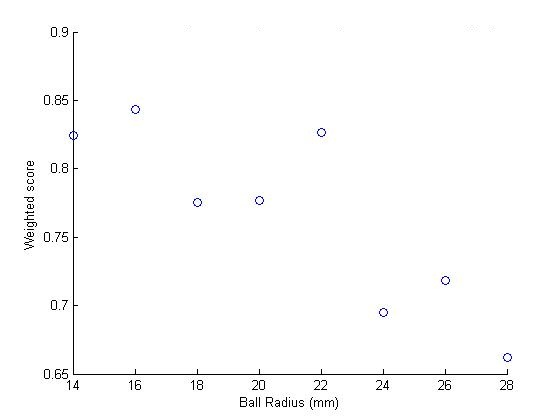
\includegraphics[width=0.5\textwidth]{figures/weightedScore.jpg}
\label{enjoyment}
\end{figure}

We see in \ref{enjoyment} that $f$ seems to decrease at increasing radius. The model seems to show that we should pick a ball around either $14\ut{mm}$ or $22\ut{mm}$ in radius. Since smaller balls are harder to see and thus may not be as suitable for television broadcast, we determine $44\ut{mm}$ to be the optimal radius. There are some obvious weaknesses here, which will be further discussed in the next section.

\subsection{Weaknesses}
There are some weaknesses to our simplified model, mostly owing to the estimation of the parameters which govern the strength of the forces at play. We go into detail in the three sections below.


\subsubsection{The Trajectory Simulation}
As indicated by \ref{spiral}, the Magnus force in itself was too powerful, even though the derivation matches literature. Hence, spin decay of the ball induced by a drag torque was considered. However, owing to the complexity of fluid dynamics, and a highly variable Reynolds number when transitioning between slow spin and fast spin, the estimated dependence of drag on the Reynolds number was likely somewhat inaccurate. We observed that at high initial angular velocities, the limit of how much the ball could change directions after the bounce, and 'curve' (by Magnus) during flight after the bounce, was less than what could be observed during a match, especially on a particularly well-delivered side-spin shot.

\subsubsection{The Monte Carlo Simulation}
Due to a time and resource constraint, we could not perform the Monte Carlo simulation for as many steps as we hoped for, and were limited to only 2000 iterations per radius. Since the simulation is four dimensional We assumed all shots were made from the edge of the table and a fixed position. Although the position itself was reasonable (roughly 40cm above the table, where most shots are taken when on the offensive in a game), it would not be representative of the whole game. But considering that the game is far slower when a player is on the defensive far behind the court, as they are often lobbing the ball back, this was not our primary concern for when to slow the game down. It as more interesting to see how the game is affected by ball size for a player on the offensive, who must hit the ball faster, (and with a wider angle) than his opponent can reach, and so this is where slowing down the game by changing the radius would have greatest effect. This would also be where most spectators would have trouble tracking the ball, considering the increase in speed during an attack rather than a defensive lob. \\

Due to the time constraints, we considered only one input energy as our radius for the Monte Carlo simulation. Several table tennis players noted that larger balls spin less \cite{ITTF-STATS}, but a ball given the same initial angular velocity would experience more lift due to Magnus (for the same perpendicular velocity), not less, since it grows with the radius. Thus the difference is in the input the players can impart to the ball, which means that their ability to impart the same speed and spin must be compromised by an increase to the size of the ball. We place a limit on the kinetic energy that can be put into the ball to account for this, so that even though a larger ball may have spin imparted to it, the amount of spin decreases due to the increase of the moment of inertia, and the decrease in the perpendicular component of the translational velocity. \\

From \ref{enjoyment}, we see that the simulations made were not enough to give us a detailed profile of $f$. Furthermore, due to the random simulation, the noise of the randomness can be easily seen in all of the simulations generated. The solution to these problems would be to run a longer simulation with larger iterations. However, we were unable to do this within the prescribed time limit, making this model potentially inaccurate.

\section{Conclusions}

From Monte Carlo simulations, we see that the game will slow down as the radius increases. Hence the $40\ut{mm}$ ball results in both a slower spin and a slower game than the $38\ut{mm}$ ball. Taking into account both the spin and the speed of the game, we determine the optimal ball size to be $44\ut{mm}$.

\bibliographystyle{amsplain}
\bibliography{simple}

}

\newpage

\onecolumn
\section{Appendix}

\subsection{Table of Values} All constants used in the paper are defined below for convenience.

\begin{tabular}{ l || c | r }
  \hline                        
  $r$                       &                                & radius of the ball in meters\\
  $m_{r}$                     &                                & mass of ball of radius r\\
  $\mb{v}$               &                                & translational velocity of ball \\
  $\boldsymbol{\omega}$       &                            & translational velocity of ball \\
  $\mb{F_{G}}$          &                                & force by gravity \\
  $\mb{F_{D}} $        &                                & force by drag \\
  $\mb{F_{M}} $      &                                & force by Magnus \\
  $g$                      & $9.8\ut{ms^{-2}}$       & acceleration by gravity \\
  $C_{D}$               & 0.5                           & drag coefficient of hollow sphere \\
  $\rho$                  & $1.225\ut{kgm^{-3}}$ & density of air \\
  $\mu$                  & 0.25                         & coefficient of kinetic friction between ball and table \\
  table length          & $2.74\ut{m} $                & length of table tennis table \\
  table width           & $1.525\ut{m} $              & width of table tennis table \\
  net height            & $0.1525\ut{m} $             & table tennis table net height \\       
  $E_{max}$          & $\frac{1}{2}m_{0.020}||\mb{v}_{avg}||^{2} $ & Input energy used, equal to kinetic energy of average speed shot with no spin. \\
  $\epsilon$ & 0.93 & coefficient of restitution \\
  \hline  
\end{tabular}



\subsection{Code}

\lstinputlisting[language=MATLAB]{SimulationCode/final_plot.m}
\lstinputlisting[language=MATLAB]{SimulationCode/all_shots.m}
\lstinputlisting[language=MATLAB]{SimulationCode/monte_carlo.m}
\lstinputlisting[language=MATLAB]{SimulationCode/simulate_shot.m}
\lstinputlisting[language=MATLAB]{SimulationCode/get_position_on_table.m}
\lstinputlisting[language=MATLAB]{SimulationCode/bounce.m}
\lstinputlisting[language=MATLAB]{SimulationCode/ball_flight_vel.m}
\lstinputlisting[language=MATLAB]{SimulationCode/ball_flight_pos.m}
\lstinputlisting[language=MATLAB]{SimulationCode/changeR.m}
\lstinputlisting[language=MATLAB]{SimulationCode/getConstant.m}



\end{document}
